\chapter*{Analysis overview}\label{chap:analyintro}

% \section{c}

Historically, signatures with dilepton final states have been central in shaping the SM, from discoveries of new particles~\cite{PhysRevLett.33.1404, PhysRevLett.33.1406,1977PhRvL..39..252H,1983398,BAGNAIA1983130}, through many precision measurements~\cite{ALEPH:2005ab,Aad:2016zzw,Aad:2016izn,Sirunyan:2018swq}, and in searches for new BSM physics~\cite{Aad:2019fac,Sirunyan:2018exx,Sirunyan:2018ipj,EXOT-2016-05}. Traditionally, the dilepton channel has been used due to its clean and fully reconstructible experimental signature with excellent detector efficiency. The following chapters outline a novel search for new non-resonant phenomena in final states with two electrons (\ee) or two muons (\mumu) at \SI{139}{\femto\barn^{-1}} of data collected in \protonproton collisions at the LHC in $\sqrt{s}=\SI{13}{\tera\electronvolt}$. This analysis complements the search for heavy resonances~\cite{Aad:2019fac} by using the same dataset and selection criteria. The non-resonant signatures have a broad deviation in the tails of the smoothly falling invariant-mass spectrum, where the main background is the irreducible Z/$\gamma^*$ (Drell-Yan, DY) process. The results are provided in a model-independent format, and is also interpreted in the context of the frequently tested benchmark Contact-interaction (CI) models. A detailed overview of the theoretical motivation for contact interaction searches was given in~\cref{chap:SM}. The \ee and \mumu invariant-mass spectrum is chosen as the main observable in the analysis as it offers the best discriminating power against signal and background for non-resonant signals like CIs. 

Several changes have been introduced in this analysis with respect to previous ATLAS results~\cite{EXOT-2016-05}. This is the first non-resonant dilepton search at the LHC to use a background estimate from a data-driven fit method instead of relying on simulation. The background at high invariant mass is estimated from a fit to a low-mass control region (CR), utilising an extrapolation procedure. The impact of MC mismodelling is significantly reduced when estimating the background using the data. Additionally, the search is performed in a high mass single-bin signal region (SR), where both the regions and the function choice are optimised to maximise the sensitivity of observing a CI process. There are four SRs used in the analysis, two SRs for the electron selection and two SRs for the muon selection. The SRs are optimised to be sensitive to the constructive and destructive interference CI models, resulting in two SRs for each channel: constructive and destructive SRs. Using the single bin approach the results are presented as  model-independent number of signal events in the SRs and also interpreted as the CI energy scale parameter $\Lambda$. The benefit of a model-independent search to facilitate the reinterpretation of the results by theorists, which allows for a wider use of the results produced by the analysis. 

The following chapters will describe the analysis strategy and results from the Run-2 ATLAS search for non-resonant phenomena using \SI{139}{\femto\barn^{-1}} of data at a $\sqrt{s}=\SI{13}{\tera\electronvolt}$. \cref{fig:nonres:intro:analysismodel} outlines the analysis model of the search. The terms in the diagrams will be explained in the following chapters. The object and event selection is described in ~\cref{chap:eventsel}. The selection is validated in terms of data/MC comparisons, where the MC samples used are outlined in~\cref{chap:datamc}. The "transfer function" described in~\cref{sec:datamc:transfer} is a parametrisation of the detector mass resolution introduced in the analysis to produce smooth MC templates, which are used to validate the functional fit. The background estimation procedure is described in~\cref{chap:bkgmodel}. An important part of the background fit model choice is understanding and estimating the uncertainties associated with it. The uncertainties are described in \cref{sec:extrap:uncertainties}. Once a function has been chosen, the optimisation procedure to pick a CR and SR are described in \cref{sec:extrap:optimisation}. The statistical analysis used is described in \cref{chap:stats}. Finally, the results are presented in~\cref{chap:results}. 

\begin{figure}[h]
    \centering
    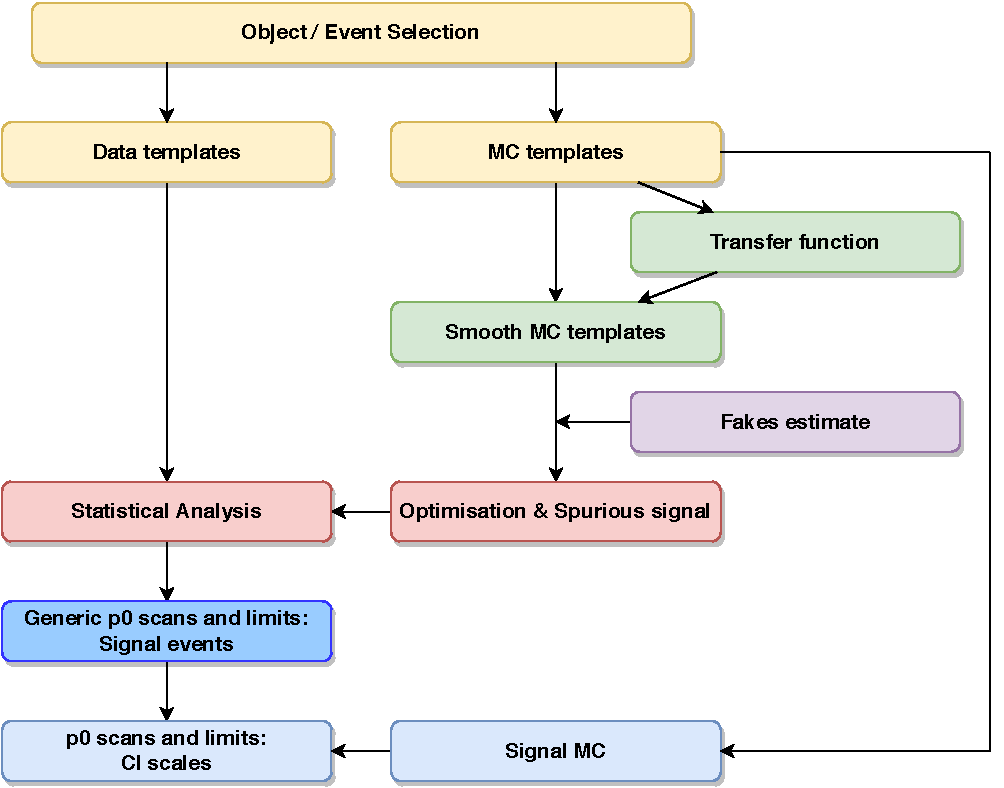
\includegraphics[width=\largefigwidth]{figures/analysis/introduction/AnalysisOverview.pdf}
    \caption[Analysis model of the full Run-2 dilepton non-resonant search]{Analysis model of the full Run-2 dilepton non-resonant search.}
    \label{fig:nonres:intro:analysismodel}
\end{figure}
\clearpage